\section{Проведение эксперимента}
В данной работе регистрация спектров поглощения паров иода производится с помощью автоматического спектрофотометра для видимой и ультрафиолетовой областей <<Specord M400>>. Оптическая схема прибора приведена на рис. \ref{fig:ust}.

\begin{figure}[h!]
\centering
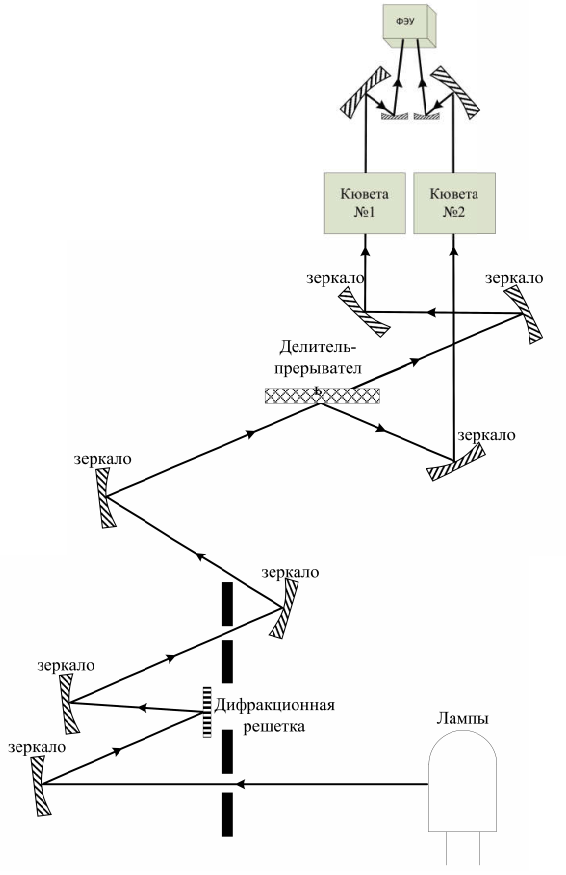
\includegraphics[width=0.6\linewidth]{ust.png}
\caption{Оптическая схема прибора}
\label{fig:ust}
\end{figure}

Для наблюдения изменения характера спектра при изменении температуры цилиндрическая стеклянная кювета с кристаллами иода устанавливается в кюветном отсеке прибора с помощью специального кюветодержателя, который нагревается до необходимой температуры водой, подаваемой по соединительным шлангам от термостата. Схема установки изображена на рис. \ref{fig:ust1}.

\begin{figure}[h!]
	\centering
	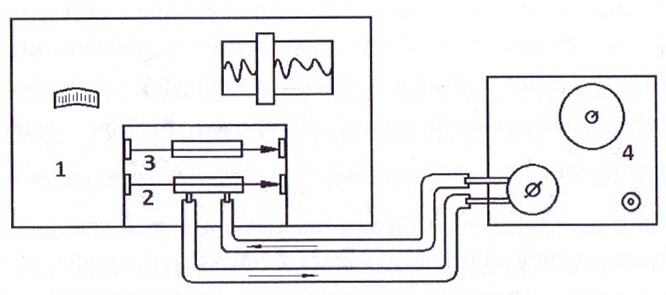
\includegraphics[width=0.4\linewidth]{ust1.jpg}
	\caption{Схема установки: 1 --- корпус спектрометра, 2 --- кювета с парами иода, 3 --- кювета сравнения, 4--- термостат}
	\label{fig:ust1}
\end{figure}

